\documentclass{article}
\usepackage{amsmath, amssymb}
\usepackage{bm}
\usepackage{graphicx} % Required for inserting images
\usepackage{tikz}
\usepackage{float}
\usepackage[round]{natbib}

\bibliographystyle{plainnat}
\usepackage[a4paper, top = 2cm,
                     bottom = 2cm,
                     left = 2cm,
                     right = 2cm]{geometry}


\title{Dynamic economic geography models and resource economics}
\author{Simon Jean}
\date{July 2023}


%%%%%%%%%%%%%%%%%%%%%%
\newcommand*{\xMin}{0}%
\newcommand*{\xMax}{5}%
\newcommand*{\yMin}{0}%
\newcommand*{\yMax}{3}%


\newtheorem{assumption}{Assumption}

\begin{document}


\maketitle

\section{General model}
I develop a 2-patch model, followed by a 3-patch model. My intuition is that the 'public good' nature of dispersal is not comprised in a 2-patch model. \\
\textit{Unclear if there is a public good nature of dispersal: on the one hand, increasing dispersal from patch A to B, if B is connected to C, increases the resource stock in the end. However, it's not really a "public" good: it is a collective, if anything, contribution, but not everyone benefits from it. }
\subsection{Resource dynamics}
I use a dynamic resource stock, with asymmetric dispersal : 
\begin{align}
    X_{1,t+1} &= d_{11,t} g_1(X_{1t}-h_{1t}) + d_{21,t}g_2(X_{2t}-h_{2t})\\
     X_{2,t+1} &= d_{22,t} g_2(X_{2t}-h_{2t}) + d_{12,t}g_1(X_{1t}-h_{1t})
\end{align}
%In the matrix form with escapement $e_t = X_t - h_t$:
%$\mathbf{X}_{t+1}=    \begin{pmatrix}
%        X_{1,t+1}\\
%        X_{2,t+1}
%    \end{pmatrix}$, $\mathbf{D}_t=\begin{pmatrix}
%        d_{11t} & d_{12t}\\
%        d_{21t} & d_{22t}
%    \end{pmatrix}$, 
%    $\mathbf{g}=\begin{pmatrix}
%        g_1()\\
%        g_2()
%    \end{pmatrix}$ and given escapement $e_t = X_t - h_t$, $\mathbf{e}_t = \begin{pmatrix}
%        e_{1t}\\
%        e_{2t}
%    \end{pmatrix}$:
    
%\begin{equation}
%    \mathbf{X}_{t+1} = \mathbf{g(e_t)}'\mathbf{D}_t
%\end{equation}

\subsection{Choice variables}
In this version of the toy model, patch owners get a net marginal benefit from harvesting a mobile resource. The model can also be turned to study invasive species or wildfires. The decision-making scale is the patch. A social planner may try to optimize the sum of patch-specific benefits, but so far, does not add any other values, such as a conservation value, or other non-market benefits. 
\subsubsection{Dispersal}
Patch owners can influence the dispersal between patches. First, patch owners can influence the dispersal from their patch $i$ to their neighbor's $j$, $d_{ij}$. The question remains open if they can \textit{attract} the resource from the neighboring patches or not. In the case of fish aggregating devices (FADs), the competition is to lure fish within the economic zone. In the case of wildfires, one can undertake defensive actions so that even if fire could spread from a neighbor, the damages could be reduced. In the case of a 'bad' species, a neighbor would want to send everything to its neighbor. Can there be defensive action? 
\\
Let's assume that : 
\begin{equation}
    d_{ij,t+1} = f_{ij}(d_{ij,t}, z_{it}, z_{jt})
\label{eq:d_ij}
\end{equation}
Equation \ref{eq:d_ij} shows that dispersal can be chosen each period, with dependence with respect to the past, such that $\frac{\partial f_{ij}}{\partial d_{ijt}}\geq 0$. Moreover, $\frac{\partial f_{ij}}{\partial z_{it}}\leq 0$ and $\frac{\partial f_{ij}}{\partial z_{jt}}\geq 0$ in the case where the resource is a good: investment by the patch owner $i$ in dispersal reduces the resource flow to its neighbor $j$, while when the neighbor increases its investment it can attract more resources from $i$ to $j$. Eventually, dispersal \textit{from $i$ to $j$} is limited by exogenous factors e.g dispersal is bounded: $0\leq m_{ij} \leq d_{ij,t} \leq M_{ij} \leq 1$.
\textit{What about second-order derivatives?}

Finally, note that each patch owner only has 1 decision variable $z_t$. This represents investments in connectivity, i.e. FADs, or own defensive space, for example. The cost of $z_t$ is increasing and convex, i.e, $c_i(.)'>0, c_i(.)"<0$ and normalized such that $c_i(0)=0$


\subsubsection{Harvesting}
Assume the resource is an economic good. 
In each patch, the resource is harvested to maximize the contemporaneous net benefits, depending on location $i$. The contemporaneous net benefits depend on the revenues from harvesting $h_t$ and from the (marginal) costs from harvesting from $X_t$ to residual stock (or escapement) $e_t = X_t - h_t$, $\omega_i(s)$: 
\begin{equation}
    \Pi_i = B_i(X_{it} - e_{it}) - \int_{e_it}^{X_{it}}\omega_i(s)ds
\end{equation}
\subsection{Model formulation}
\subsubsection{Social planner}
The goal of the social planner is to maximize the discounted sum of profits over the landscape and time : 
\begin{align*}
    \max_{\{e_{it}, z_{it}\}_{i\in \{1,2\}}} & \sum_{t=0}^T \beta^t \left( \sum_{i=1}^2 B_i(X_{it} - e_{it}) - \int_{e_it}^{X_{it}}\omega_i(s)ds - c_i(z_{it}) \right)\\
    &\text{Such that:}\\
        d_{ij,t+1} &= f_{ij}(d_{ij,t}, z_{it}, z_{jt})\\
         X_{1,t+1} &= d_{11,t} g_1(e_{1t}) + d_{21,t}g_2(e_{2t})\\
     X_{2,t+1} &= d_{22,t} g_2(e_{2t}) + d_{12,t}g_1(e_{1t})
\end{align*}
\section{Toy model}
In this model, I keep the same overall structure, but I simplify the objective function. I assume that prices are uniformly distributed across patches and constant marginal costs are heterogeneous such that the net marginal benefit from harvesting is $p_i$. The goal of the social planner is to maximize the discounted sum of profits over the landscape and time : 
\begin{align*}
    \max_{\{e_{it}, z_{it}\}_{i\in \{1,2\}}} & \sum_{t=0}^T \delta^t \left( \sum_{i=1}^2 p_i(X_{it} - e_{it}) - c_i(z_{it}) \right)\\
    &\text{Such that:}\\
        d_{ij,t+1} &= f_{ij}(d_{ij,t}, z_{it}, z_{jt}) \text{ for } i,j \in 1,2\\
         X_{1,t+1} &= d_{11,t} g_1(e_{1t}) + d_{21,t}g_2(e_{2t})\\
     X_{2,t+1} &= d_{22,t} g_2(e_{2t}) + d_{12,t}g_1(e_{1t})
\end{align*}

\subsection{Using backward induction to get a glimpse into the policy function}
Let $T$ be the end of the planning horizon, such that $V_{T+1}(X_{T+1},D_{T+1})=0$. In this case, because extraction is costless, and there is no tomorrow, $e_{iT} = 0$. Moreover, because investments in connectivity will not yield any return, $z_{iT}=0$. Therefore, $V_T(X_T,D_T)=p_1 X_{1T}+p_2 X_{2T}$. 
\\
Turn to the optimization in $T-1$:
\begin{align*}
    V_{T-1}(X_{T-1}, D_{T-1}) &= \sum_{i=1}^2\left(p_i(X_{iT-1}-e_{iT-1}) - c_i(z_{iT-1} )\right) + \delta V_T(X_T, D_T)\\
    &= \sum_{i=1}^2\left(p_i(X_{iT-1}-e_{iT-1}) - c_i(z_{iT-1} )\right) + \delta\left[ \sum_{i=1}^2 p_i \left( \sum_{j=1}^2 d_{jiT}g_j(e_{jT-1})\right)\right]\\
    &= \sum_{i=1}^2\left(p_i(X_{iT-1}-e_{iT-1}) - c_i(z_{iT-1} )\right) +  \delta \left[ \sum_{i=1}^2 p_i \left( \sum_{j=1}^2 f_{ji}(d_{ji},z_{jT-1},z_{iT-1})g_j(e_{jT-1})\right)\right]&\\
\end{align*}
Now, use the fact that $\sum_{j=1}^N f_{ij}(d_{ij}, z_{it},z_{jt})=1$, so that $f_{ii}(d_{ii},z_{jT-1},z_{jT-1})=1 - \sum_{j\neq i}f_{ij}(d_{ij}, z_{it},z_{jt})$:
\begin{equation}
    V_{T-1}(X_{T-1},D_{T-1})=\sum_{i=1}^2\left(p_i(X_{iT-1}-e_{iT-1}) - c_i(z_{iT-1} )\right) + \delta \left[ \sum_{i,j,i \neq j} p_i \big( f_{ji}(\cdot,\cdot,\cdot) g_j(e_{jT-1}) + (1 - f_{ij}(\cdot,\cdot,\cdot)g_i(e_{iT-1})\big)\right]
\end{equation}
First-order conditions are : 
\begin{equation}
\frac{\partial V_{T-1}}{\partial e_{iT-1}} = 0 \iff g'_i(e_{iT-1}) = \frac{p_i}{\delta [p_i(1- f_{ij}(\cdot,\cdot,\cdot)) + p_j f_{ij}(\cdot,\cdot,\cdot)]}
\label{eq:e_t}
\end{equation}
This result is canonical: optimal harvest in patch $i$ should be such that the current marginal benefit in patch $i$, $p_i$, equals the discounted future marginal benefit of harvesting the resource in the patches where it migrates. It boils down to the golden rule when there is no spatial interaction (i.e. when $f_{ij}(.,.,.) =  0$).

\subsubsection{Insights into connectivity investment}
For an interior solution regarding investments in connectivity (i.e $z_{iT-1}>0$):
\begin{equation}
    \frac{\partial V_{T-1}}{\partial z_{iT-1}}= 0 \iff c'_i(z_{iT-1}) = \delta (p_i - p_j)\left[
    \frac{\partial f_{21}}{\partial z_{iT-1}} g_2(e_{2T-1}) - \frac{\partial f_{12}}{\partial z_{iT-1}}g_1(e_{1T-1})
    \right]
    \label{eq:z_t}
\end{equation}
Focus on patch 1 and suppose it has a lower marginal cost of harvesting than patch 2, such that $p_1 > p_2$.
Assume that connectivity investment \textit{only has a defensive impact}, i.e $\frac{\partial f_{ij}}{\partial z_i}\leq 0$ and $\frac{\partial f_{ij}}{z_j}=0$. Then, the optimal investment is such that :

$$
c'_1(z_{1T-1}) = \delta (p_1 - p_2)\left[ - \frac{\partial f_{12}}{\partial z_{1T-1}}g_1(e_{1T-1})
    \right]
$$
In other words, the owner of patch $i$ invests up to the point where the current marginal cost of connectivity $c'_i(z_{iT-1})$ equals the discounted future marginal profit, and ultimately depends on the extraction rate in patch 1. The larger the gap in prices across space and the efficiency of connectivity investment at reducing leakage \textbf{from} patch 1, the larger the investment. 
\\\\
Now assume that connectivity investment \textit{only has an aggressive impact}, i.e $\frac{\partial f_{ij}}{\partial z_i} =  0$ and $\frac{\partial f_{ij}}{z_j}\geq 0$. 
$$
c'_1(z_{1T-1}) = \delta (p_1 - p_2)\left[ \frac{\partial f_{21}}{\partial z_{1T-1}}g_2(e_{2T-1})
    \right]
$$
In this case, investment is such that the current marginal cost equals the discounted future marginal benefits, in the form of the net increase in marginal profit caused by the price differential and the increase in quantity sold in patch $1$, from displacing the resource from patch 1 to 2. 

Now assume investment in connectivity has both \textit{an aggressive and defensive impact} i.e, it reduces the outflow of resources from patch 1 to patch 2 and increases the inflow from patch 2 to patch 1. The level of investment depends on the difference in earnings between the two patches. Given that the price level is larger in patch 1, the combined effects imply an even larger investment in connectivity. 

\subsubsection{Properties of the system}
Contrary to the system described in \cite{costello_optimal_2008} and in the class notes, I don't think the solution found here is state-independent. The escapement 'trick', in the case of an interior solution, guarantees state independence in this setup. On the other hand, if the dynamics of dispersal follow equation \ref{eq:d_ij}, there is a clear state dependence, where $\mathbf{e_t}$ and $\mathbf{z_t}$ will eventually depend on $\mathbf{D_t}$. 

One way to circumvent the problem could be to find an 'escapement trick' analogous to \cite{costello_optimal_2008} for dispersal choice, in the case of an interior solution for dispersal investment. Escapement measures a residual stock and is related to harvesting through a simple linear equation. There are two main obstacles to such an approach : 
\begin{enumerate}
    \item \textit{Nonbijective nature of the relationship (from non-injectivity)}\\
    In the case of the escapement trick, once the space given by $X$ is given, there is a bijection between the remaining stock $e$ and the harvest $h$. In my case, once the original level of connectivity is given, the variation depends on two flows. Difficult to have a bijection from a social planner perspective, however, it may be easier from a game theoretic perspective when taking the existing rate of dispersal as given, and the actions from a competitor. \\
    \textbf{After more thought:} $\mathbb{R}^2$ is 'richer' than $\mathbb{R}$ : a function from the former to the latter will never be invertible. The only way to reach invertibility is to make sure the dimensions between each space are identical.
    \begin{itemize}
        \item Dispersal flows are bilateral issues: a neighbor who is not connected to me cannot influence my connection with my neighbor \textit{directly}. What can matter is therefore the relative efficiency of investment to direct flows, in asymmetric functions, with boundary conditions.\\
        Idea : 
        \begin{align*}
        f: \mathbb{R} &\rightarrow \mathbb{R}\\
            \frac{z_{it}}{z_{jt}} &\mapsto f\left(\frac{z_{it}}{z_{jt}}\right)
        \end{align*}
        And in the end, I think if I have something like :
        $$
        d_{ijt+1} = \phi(d_{ijt}) + f(z_{it}, z_{jt})
        $$
        It can be invertible!\\
       \item \textbf{ An issue remains with the double definition} of the ratio maybe, with the issue that the ratio is pinned down twice, by $f_{ij}$ and $f_{ji}$
        \\
        If I define flows as a bilateral phenomenon, there is a notion of symmetry that is implied; however, for some reason, it may be easier to go from A to B than from B to A. At the same time, it should be possible to make dispersal endogenous. I wonder if maybe the conditions for the double effect (i.e, defense and baiting) should be different when it comes to $\sum_j d_{ij}$. 
        \item Maybe it should be that $\frac{z_i}{z_j}$ defines the net flow between $i$ and $j$ such that $-1 \leq d_{ij} \leq 1$ overall. In this case, $\sum_j \sum_i d_{ij}=n$ becomes the boundary condition, and further restrictions apply, that are difficult to put in a smooth calculation framework : the net flow is limited by the 
    \end{itemize}
    \item \textit{Expressing the key phenomenon with a different statistic}\\
    If I restrict the effects of connectivity investment so that dispersal from one patch to another only depends on one choice variable. I can then design a variable such that what matters is the change in connectivity, for example :
    \begin{align*}
        d_{ijt+1} = f( z_{it}+d_{ijt}) \Rightarrow z_{it} = f^{-1}(d_{ijt+1})-d_{ijt}
    \end{align*}
    The question remains as to how to express the dynamics of $\mathbf{X_t}$ with the new and improved $z_{it}$ and without dependence on $d_{ijt}$
\end{enumerate}
An idea is : 
\begin{equation}
    d_{ijt+1} = [a_i - \delta d_{ijt}] + \frac{b_i - a_i}{1-\exp(-f_{ij}(z_{it},z_{jt}))}
\end{equation}
\\\\
Another avenue would be to check if there is a notion of 'partial state independence', that could at least simplify the problem. 



\subsubsection{Are connectivity and harvest substitutes or complements? }
One of the key insights from equations \ref{eq:e_t} and \ref{eq:z_t} is that they both determine the system optimum. In other words, unless prices and marginal costs are uniformly distributed on the landscape, the optimal harvest rule is different when dispersal can be made endogenous. How do the two interplay? 

In the exogenous dispersal, state-independent, version of this problem, optimal escapement can (implicitly) be redefined from equation \ref{eq:e_t} as : 
$$
g'_i(e_{iT-1}) \delta[(p_j - p_i)f_{ij}(d_{ijT-1}, z_{iT-1}, z_{jT-1}) + p_i] = p_i
$$

To study the behavior of the two solutions, I would need stronger assumptions on the second derivative of all the functions, and a better understanding of the behavior of $g$. I can add more structure to the model for theoretical insight. 

\textit{Let's make a thought experiment:}\\
Assume I deal with the two patches, up in the future. I know there is a price differential between the two patches. I have a decision to make: should I increase the dispersal between patches, or not, and at what expense? In order to make more profit tomorrow, I could reshuffle all my assets to the most profitable area. However, reshuffling is costly. To maintain profits, I would need to increase the extraction rate today, so that I could invest in dispersal tomorrow. However, doing so may reduce the profits tomorrow, even though there is more connectivity: I have pipes, but no water to go through, I have ecoducts, but no animals to guide across the road. Could it be that I increase extraction today, to maintain connectivity in the future? That would be reasonable if the discounted future stream of revenues from reshuffling and over-harvesting currently outweighs the current costs of reshuffling. I might even keep on investing, or maintain the state of the investment if it makes the resource more profitable in time. My intuition is there is some complementarity of connectivity and harvesting in the most valuable patches, while it may not be the case for other patches; 

\subsection{Imposing more structure on dispersal}
I focus on a renewable resource, not just the spread of a phenomenon (that'll come next). Therefore, I set as the first assumption that :
\begin{assumption}
    $d_{ijt}$ represents the share of resource that disperses from patch $i$ to $j$ in period $t$. Therefore : 
    \begin{align*}
    &0 \leq d_{ijt} \leq 1\\
    &\sum_{j=1}^N d_{ijt}=1
    \end{align*}
\end{assumption}
\newpage

\section{Fences and baits}
\subsection{Motivation}
Assume I have a renewable resource whose habitat spans several land patches. The resource freely flows across patches according to some biological, exogenous determinants.  Assume we have 2 patches, A and B, such that the net benefit of harvest in A is larger than in B (people in A may love the resource, while in B they just like it; they may also be more efficient at harvesting it than in B). As people in A do love their resources, they may be tempted to ensure they stay in A and fence their land. They also notice that B has resources, and are tempted to increase the migration flow from B to A, and bait the resource into A. \\\\
The question that emerges is: how does the harvest of a renewable resource change when fencing and baiting are considered?

\subsection{Modeling strategy}
\subsubsection{A 2 patch model}
In each period and each patch, the resource stock $X_{At}$ and $ X_{Bt}$ is harvested at $h_{At}$ and $h_{Bt}$, leaving a remaining stock $e_{At}$ and $ e_{Bt}$ which then grows to $g_A(e_{At})$ and $g_B(e_{Bt})$, with $g'_i()>0$ and $g''_i()<0$. Once it grows, it migrates. For example, in patch $A$, a share $d_{AAt}$ of the stock remains in $A$ in period $t$, while a share $d_{ABt} = 1-d_{AAt}$ flows from $A$ to $B$, and reciprocally for $B$. At the beginning of period $t+1$ : 
\begin{align}
    X_{At+1} = (1-d_{ABt})g_A(e_{At})+d_{BAt}g_B(e_{Bt})
    \\
    X_{Bt+1} = (1 - d_{BAt})g_B(e_{BT}) + d_{ABt}g_A(e_{At})
\end{align}

In each period, after observing the dispersal flows, landowners choose whether to improve their fences, increase the baiting, or further improve their land. 
Dispersal in the next period will depend on each landowner's fencing $z_{At}^F$and $z_{Bt}^F$ and baiting and land improvement practices $z_{At}^B$ and $z_{Bt}^B$, as well as historical dispersal $d_{ABt}$, and natural, exogenous features that limit dispersal : 
\begin{align}
    d_{ABt+1} = f_{AB}(z^F_{At}, z^B_{Bt}, d_{ABt}) \in [m_{AB},M_{AB}] \subset [0,1] \\
    d_{BAt+1} = f_{BA}(z^F_{Bt}, z^B_{At}, d_{BAt}) \in [m_{BA},M_{BA}] \subset [0,1]
\end{align}
The more one landowner fences, the more it retains the resource. However, fencing is less and less effective at retaining the resources\footnote{It may be good to go back to this hypothesis: the effect of incomplete fencing may be concave, but convex at the end when the fence is finished}. Baiting increases the flow of dispersal from the neighboring patch at a decreasing rate as well. 

Eventually, baiting reduces the marginal effect of fencing and fencing reduces the marginal effect of baiting. Overall : 
\begin{align*}
    \frac{\partial f_{AB}}{\partial z^F_{At}}\leq 0 &\text{ and } \frac{\partial^2 f_{AB}}{\partial (z^F_{At})^2} \geq 0\\
    \frac{\partial f_{AB}}{\partial z^B_{Bt}}\geq 0 &\text{ and } \frac{\partial^2 f_{AB}}{\partial (z^B_{Bt})^2} \leq 0\\
    \frac{\partial ^2 f_{AB}}{\partial z_{Bt}^B\partial z_{At}^F} \leq 0 &\text{ and } \frac{\partial ^2 f_{AB}}{\partial z_{At}^F\partial z_{Bt}^B} \leq 0
\end{align*}

The timing of the model is synthetized in figure \ref{fig:timing}.

\begin{figure}[H]
  \centering
  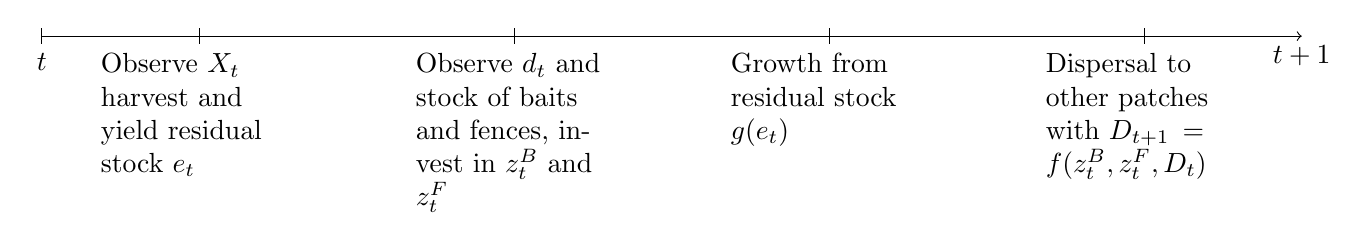
\begin{tikzpicture}
    % Draw the arrow
    \draw[->] (0,0) -- (16,0) node[anchor=north] {$t+1$};
    % Draw ticks and labels
    \draw (0, .1)--(0,-.1) node[anchor = north]{$t$};
    \draw (2, .1)--(2,-.1) node[anchor = north, text width = 2.5cm]{Observe $X_t$ harvest and yield residual stock $e_t$};
    \draw (6, .1)--(6,-.1) node[anchor = north, text width = 2.5cm] {Observe $d_t$ and stock of baits and fences, invest in $z_t^B$ and $z_t^F$};
    \draw (10, .1)--(10,-.1) node[anchor = north, text width = 2.5cm]{Growth from residual stock $g(e_t)$};
    \draw (14,.1)--(14,-.1) node[anchor = north, text width = 2.5cm]{Dispersal to other patches with $D_{t+1}=f(z_t^B, z_t^F, D_t)$};
  \end{tikzpicture}
  \caption{Timing of the model}
  \label{fig:timing}
\end{figure}

\subsubsection{Model formulation}
Landowners locally harvest the resource at a \textit{constant unit marginal cost} $\omega_i$ and sell it on a competitive market at price $p$, so the net marginal benefit is heterogeneous and can be written as $p_i = p - c_i$. Moreover, they choose fencing and baiting expenditures with costs $c_{i,l}(z_{it}^F)$ such that $c'_{i,l}\geq 0$ and $c''_{i,l} \geq 0$, and normalized such that $c_{i,l}(0) = 0$. The profit flow at time $t$ is
\begin{equation}
    \Pi_{it} = p_i(X_{it} - e_{it}) - c_{i,F}(z_{it}^F) - c_{i,B}(z_{it}^B)
\end{equation}

First, I'm interested in the social planner's problem, i.e, to maximize the intertemporal sum of discounted profits:
\begin{align*}
    \max_{\{e_{it}, z_{it}^F, z_{it}^B \}_{i \in \{A,B\}}} & \sum_{t=0}^T \delta^t \left( \sum_{i \in \{A,B\}} p_i(X_{it} - e_{it}) - c_{iF}(z_{it}^F) - c_{iB}(z_{it}^B) \right)\\
     &\text{Such that:}\\
        X_{At+1} &= (1-d_{ABt})g_A(e_{At})+d_{BAt}g_B(e_{Bt})
    \\
    X_{Bt+1} &= (1 - d_{BAt})g_B(e_{BT}) + d_{ABt}g_A(e_{At})\\
     d_{ABt+1} &= f_{AB}(z^F_{At}, z^B_{Bt}, d_{ABt}) \\
    d_{BAt+1} &= f_{BA}(z^F_{Bt}, z^B_{At}, d_{BAt})
\end{align*}
\subsection{Model resolution and insights}
First, due to the recursive nature of the problem, if a solution exists, we can write the Bellman equation : 

\begin{equation}
    V(\mathbf{X}_t, \mathbf{D}_t) = \max_{\{e_{it}, z_{it}^F, z_{it}^B\}_{i \in \{A,B\}}} \sum_{i \in \{A,B\}} p_i(X_{it} - e_{it}) - c_{iF}(z_{it}^F) - c_{iB}(z_{it}^B) + \delta V(\mathbf{X}_{t+1}, \mathbf{D}_{t+1})
\end{equation}
\subsubsection{Using backward induction}
As $T$ is the end of the planning horizon, any resource left over in $T+1$ will have no value. Therefore, the optimal policies in $T$ are to exhaust the existing stocks, and not to invest in connectivity, i.e $e_{AT}=e_{BT}=z_{AT}^F = z_{AT}^B = z_{BT}^F = z_{BT}^B$, and the value function in $T$ is :
$$
V_T(\mathbf{X}_T, \mathbf{D}_T) = p_A X_{AT} + p_B X_{BT}
$$

Therefore, in $T-1$:
\begin{align*}
    V_{T-1}(\mathbf{X}_{T-1}, \mathbf{D}_{T-1}) = \max_{\{e_{iT-1}, z_{iT-1}^F, z_{iT-1}^B \}_{i \in \{A,B\}}} \sum_{i \in \{A,B\}} & p_i(X_{iT-1} - e_{iT-1}) - c_{iF}(z_{iT-1}^F) - c_{iB}(z_{iT-1}^B) \\&+ \delta (p_A X_{AT} + p_B X_{BT})
\end{align*}
Using the laws of motion of dispersal and the resource, I get the following first-order conditions for interior solutions of $\{e_{AT-1}, e_{BT-1}, z_{AT-1}^F, z_{AT-1}^B, z_{BT-1}^F, z_{BT-1}^B\}$:
\begin{align}
    \frac{\partial V_{T-1}}{\partial e_{AT-1}} = 0 &\Rightarrow g'_A(e_{AT-1}) = \frac{p_A}{\delta (p_A (1-f_{AB}(z_{AT-1}^F, z_{BT-1}^B, d_{AB}))+ p_B f_{AB}(z_{AT-1}^F, z_{BT-1}^B, d_{AB})} \label{eq:foc_e}\\
    \frac{\partial V_{T-1}}{\partial z_{AT-1}^B} = 0 &\Rightarrow c'_{AB}(z_{AT-1}^B) = \delta (p_A - p_B) g_B(e_{BT-1} )\frac{\partial f_{BA}}{\partial z_{AT-1}^B} \label{eq:foc_baiting}\\
    \frac{\partial V_{T-1}}{\partial z_{AT-1}^F} = 0 &\Rightarrow c'_{AF}(z_{AT-1}^F) = \delta (p_B - p_A) g_A(e_{AT-1} )\frac{\partial f_{AB}}{\partial z_{AT-1}^F} \label{eq:foc_fencing}
\end{align}
And the same sort of expression holds for $B$. \\\\
First, equation \ref{eq:foc_e} is reminiscent of \cite{costello_optimal_2008}, and carries the same sort of intuition. However, given that dispersal is itself a state variable, it appears that optimal escapement will \textbf{not} be state-independent. \\
Equation \ref{eq:foc_baiting} carries some interesting properties: for positive baiting to be an optimal strategy (i.e. $c'_{AB}()>0$), it must be that the resource is more valuable in $A$ than in $B$. In this set-up, the value component of the marginal benefit (i.e. $\delta (p_A - p_B)$) is independent of baiting, but the volume component changes with baiting (i.e $g_B(e_{BT-1})\frac{\partial f_{BA}}{\partial z_{AT-1}^B}$). Equation \ref{eq:foc_fencing} shows that, for some positive fencing to occur, the value of the resource must be larger in $A$ than in $B$ as well. \\\\
The solution to the system is complicated to get. However, some insights emerge from the set of first-order conditions.\\
First, notice that some corner results emerge. For example, assume that the net marginal benefit in $B$ is larger than in $A$ (i.e. $p_A>p_B$). In this case, the right-hand side of equations \ref{eq:foc_baiting} and \ref{eq:foc_fencing} are negative, and $z_{AT-1}^B = z_{AT-1}^F=0$. In this case, the optimal solution is to direct the resource flow towards $B$ as much as economically rational. \\

Second, note that harvesting, fencing and baiting are jointly determined: using equation (15), one can define $e_{iT-1}=\Phi_i(z_{AT-1}^F, z_{BT-1}^B)$, with $\Phi_i = g'^{(-1)}_i(RHS)$, and $RHS$ the right-hand side of equation (15). In the end, a general (?) solution may emerge from a 4 equations system. \\
\subsubsection{A recurrence solution in an infinite horizon}
In this section, I explore the value function at any given point $t$ in time such that $t<T-1$, when the planning horizon is extended towards $T \to \infty$.
\\\\
For interior solutions to exist for $\{e_{At}, e_{Bt}, z_{At}^F, z_{At}^B, z_{Bt}^F, z_{Bt}^B\}$

\newpage
\bibliography{resources}
\end{document}
